\chapter{Existing solutions}
The urban data visualization process can be viewed from multiple perspectives. We can consider the actual physical form of the presentation --- the medium and the the interaction mechanism. On the other hand, it is possible to consider the tools used for the visualization creation, which is more closely related to the standard visualization pipeline. Considering the physical form of the visualization, the examples listed in this chapter can be divided into categories --- purely virtual visualizations, and visualizations with physical components.

\section{Visualization Tools with Physical Components}
This section presents a selected list of visualization tools and projects which use interactive physical components in any shape or form. Due to the nature of these tools, the environment where the visualization is presented plays an important role. It has a profound influence on accessibility, interactivity, and the overall user experience. All presented examples share a common scheme --- a table with interactive physical components is accompanied by a wide-screen projection presenting the actual visualization.   


\begin{figure}[h]
    \centering
    \begin{subfigure}{0.5\linewidth}
        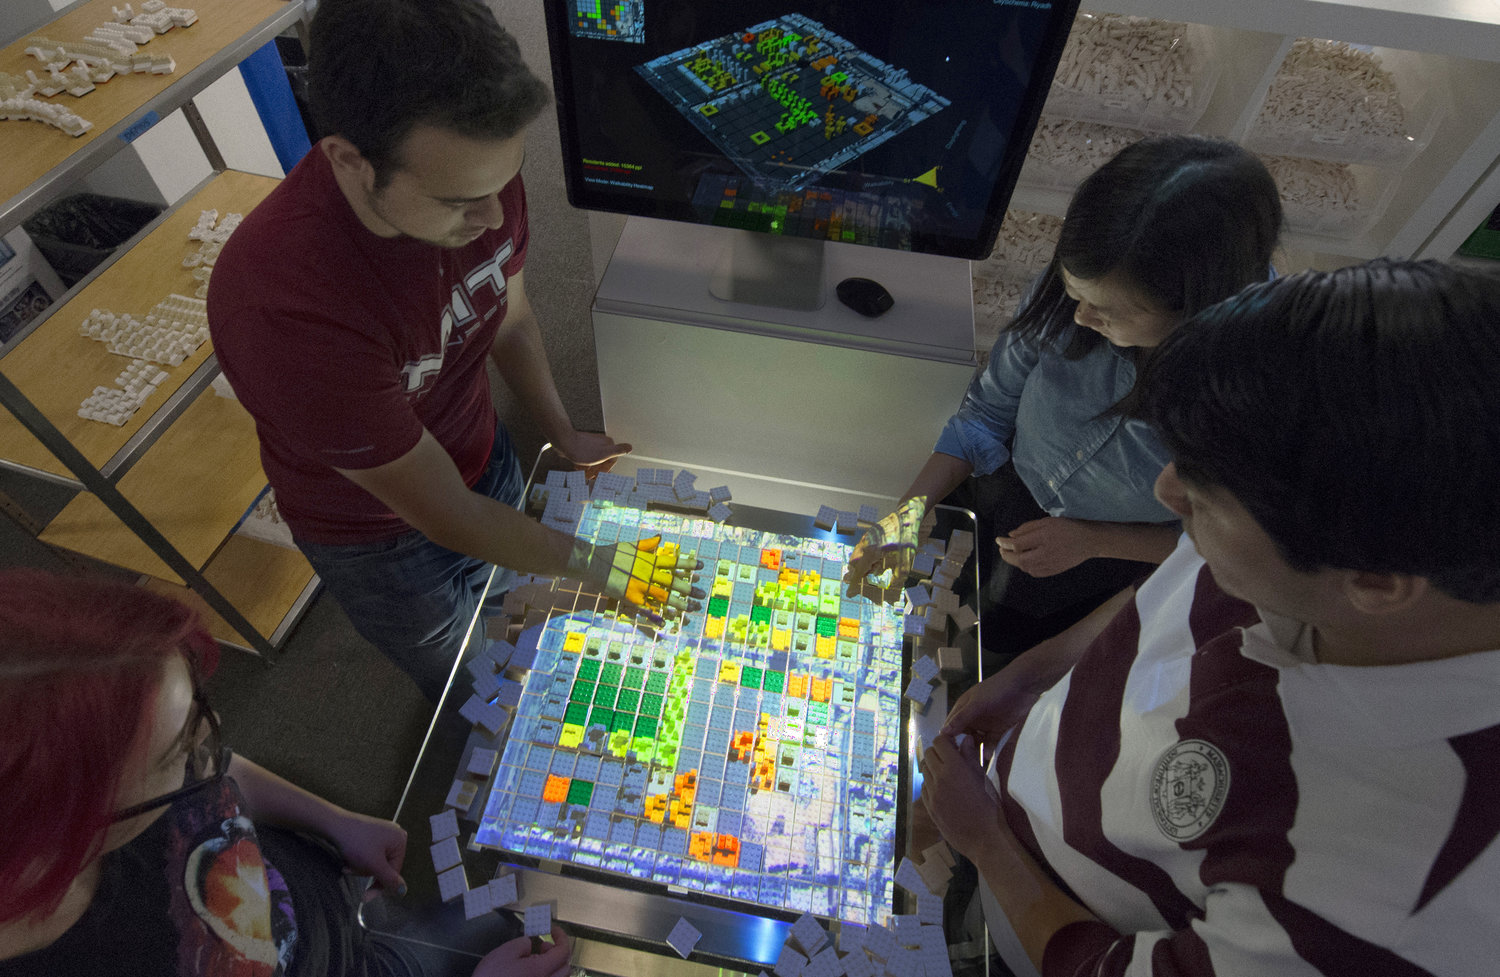
\includegraphics[width=\linewidth]{figures/tactile.jpg}
        \caption{Participants using Tactile Matrix}
    \end{subfigure}
    \begin{subfigure}{0.35\linewidth}
        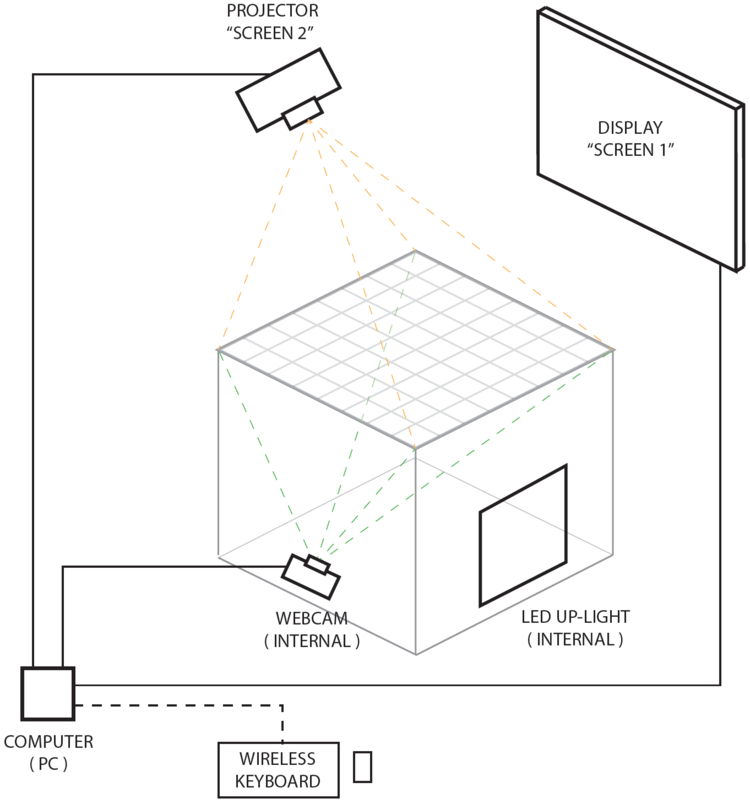
\includegraphics[width=\linewidth]{figures/tactilematrixelectronics.png}
        \caption{Scheme of the Tactile Matrix system}
    \end{subfigure}
    \caption{Tactile Matrix framework}
    \label{fig:tactilematrix}
\end{figure}

\paragraph{Tactile Matrix}
Ira Winder and Kent Larson have presented a framework called Tactile Matrix \cite{winderTangible2017}. It is a collaborative tool for real-time computation and projection mapping, see figure \ref{fig:tactilematrix}. The tool is based on a principle described in section \ref{sec:analytics}. The users are presented with a matrix representing city blocks; additional information is conveyed by the visualization projected on top of the matrix. The visualization is driven by an analytical model, which takes the matrix configuration as an input. Lego blocks can be placed into the matrix and the system updates the projection, as the model responds to new inputs. The tool is implemented in Processing, which is a Java-based environment. The SDK for the Tactile Matrix project is available, which also includes the manual to construct the physical components.




\section{Purely Virtual Visualization Tools}



